%%%%%%%%%%%%  Generated using docx2latex.pythonanywhere.com  %%%%%%%%%%%%%%


\documentclass[a4paper,12pt]{report}

% Other options in place of 'report' are 1)article 2)book 3)letter
% Other options in place of 'a4paper' are 1)a5paper 2)b5paper 3)letterpaper 4)legalpaper 5)executivepaper


 %%%%%%%%%%%%  Include Packages  %%%%%%%%%%%%%%


\usepackage{amsmath}
\usepackage{latexsym}
\usepackage{amsfonts}
\usepackage{amssymb}
\usepackage{graphicx}
\usepackage{txfonts}
\usepackage{wasysym}
\usepackage{enumitem}
\usepackage{adjustbox}
\usepackage{ragged2e}
\usepackage{tabularx}
\usepackage{changepage}
\usepackage{setspace}
\usepackage{hhline}
\usepackage{multicol}
\usepackage{float}
\usepackage{multirow}
\usepackage{makecell}
\usepackage{fancyhdr}
\usepackage[toc,page]{appendix}
\usepackage[utf8]{inputenc}
\usepackage[T1]{fontenc}
\usepackage{hyperref}


 %%%%%%%%%%%%  Define Colors For Hyperlinks  %%%%%%%%%%%%%%


\hypersetup{
colorlinks=true,
linkcolor=blue,
filecolor=magenta,
urlcolor=cyan,
}
\urlstyle{same}


 %%%%%%%%%%%%  Set Depths for Sections  %%%%%%%%%%%%%%

% 1) Section
% 1.1) SubSection
% 1.1.1) SubSubSection
% 1.1.1.1) Paragraph
% 1.1.1.1.1) Subparagraph


\setcounter{tocdepth}{5}
\setcounter{secnumdepth}{5}


 %%%%%%%%%%%%  Set Page Margins  %%%%%%%%%%%%%%


\usepackage[a4paper,bindingoffset=0.2in,headsep=0.5cm,left=1.0in,right=1.0in,bottom=2cm,top=2cm,headheight=2cm]{geometry}
\everymath{\displaystyle}


 %%%%%%%%%%%%  Set Depths for Nested Lists created by \begin{enumerate}  %%%%%%%%%%%%%%


\setlistdepth{9}
\newlist{myEnumerate}{enumerate}{9}
	\setlist[myEnumerate,1]{label=\arabic*)}
	\setlist[myEnumerate,2]{label=\alph*)}
	\setlist[myEnumerate,3]{label=(\roman*)}
	\setlist[myEnumerate,4]{label=(\arabic*)}
	\setlist[myEnumerate,5]{label=(\Alph*)}
	\setlist[myEnumerate,6]{label=(\Roman*)}
	\setlist[myEnumerate,7]{label=\arabic*}
	\setlist[myEnumerate,8]{label=\alph*}
	\setlist[myEnumerate,9]{label=\roman*}

\renewlist{itemize}{itemize}{9}
	\setlist[itemize]{label=$\cdot$}
	\setlist[itemize,1]{label=\textbullet}
	\setlist[itemize,2]{label=$\circ$}
	\setlist[itemize,3]{label=$\ast$}
	\setlist[itemize,4]{label=$\dagger$}
	\setlist[itemize,5]{label=$\triangleright$}
	\setlist[itemize,6]{label=$\bigstar$}
	\setlist[itemize,7]{label=$\blacklozenge$}
	\setlist[itemize,8]{label=$\prime$}



 %%%%%%%%%%%%  Header here  %%%%%%%%%%%%%%


\pagestyle{fancy}
\fancyhf{}


 %%%%%%%%%%%%  Footer here  %%%%%%%%%%%%%%




 %%%%%%%%%%%%  Print Page Numbers  %%%%%%%%%%%%%%


\rfoot{\thepage}


 %%%%%%%%%%%%  This sets linespacing (verticle gap between Lines) Default=1 %%%%%%%%%%%%%%


\setstretch{1.08}


 %%%%%%%%%%%%  Document Code starts here %%%%%%%%%%%%%%


\begin{document}
\sloppy
\begin{center}{\fontsize{14pt}{14pt}\selectfont \textbf{SENDING EMAIL} \\}\end{center} \par
Mail Server adalah perangkat lunak program yang mendistribusikan file atau informasi sebagai respons atas permintaan yang dikirim via email, mail server juga digunakan pada bitnet untuk menyediakan layanan serupa ftp. Selain itu mail server juga dapat dikatakan sebagai aplikasi yang digunakan untuk penginstalan email.  \par
\vspace{12pt}
\begin{center}

 %%%%%%%%%%%%  Figure/Image No:1 here %%%%%%%%%%%%%%


\begin{figure}[H]
\begin{center}
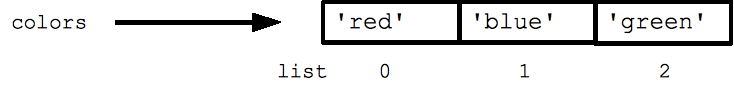
\includegraphics[width=4.65in,height=3.26in]{./uploads_new/SENDING_EMAIL.docx_DIR/media/image1.JPG}
\end{center}
\end{figure}


 %%%%%%%%%%%%  Figure/Image No:1 Ends Here %%%%%%%%%%%%%%


\end{center}\vspace{12pt}
\vspace{12pt}
Mail Server juga bisa disebut sebagai sebuah komputer yang didedikasikan untuk menjalankan jenis aplikasi perangkat lunak komputer, hal ini dianggap sebagai bagian terpenting dari setiap email sistem. Mail Server biasanya dikelola oleh seorang yang biasanya dipanggil post master. \par
\vspace{12pt}
\noindent 
Tugas Post Master  \par
\noindent 
\begin{itemize}
\item Mengelola Account \par
\noindent 
\item Memonitor Kinerja Server \par
\noindent 
\item Tugas Administratif Lainnya\end{itemize}
 \par
\vspace{12pt}
\noindent 
\textbf{Protokol Pada Mail Server} \par
\noindent 
Protokol yang umum digunakan antara lain protokol SMTP, POP3 dan IMAP. \par
\noindent 
\begin{myEnumerate}
\item SMTP (Simple Mail Transfer Protocol) \par
SMTP (Simple Mail Transfer Protocol) digunakan sebagai standar untuk menampung dan mendistribusikan email. \par
\vspace{12pt}
Simple Mail Transfer Protocol atau SMTP digunakan untuk berkomunikasi dengan server guna mengirimkan email dari lokal email ke server, sebelum akhirnya dikirimkan ke server email penerima. Proses ini dikontrol dengan Mail Transfer Agent (MTA) yang ada dalam server email Anda. Port SMTP Default: \par
\noindent 
\begin{itemize}
\item Port~25 –  Port tanpa dienkripsi \par
\noindent 
\item Port 426 – Port SSL/TLS, nama lainnya SMTPS\end{itemize}
 \par
\vspace{12pt}
\noindent 
\item POP3 (Post Office Protocol v3) \par
POP3 (Post Office Protocol v3) dan IMAP (Internet Mail Application Protocol) digunakan agar user dapat mengambil dan membaca email secara remote yaitu tidak perlu login ke dalam sistem shelll mesin mail server tetapi cukup menguhubungi port tertentu dengan mail client yang mengimplementasikan protocol POP3 dan IMAP. \par
POP3 (Post Office Protocol 3) adalah versi terbaru dari protokol standar untuk menerima email. POP3 merupakan protokol client/server dimana email dikirimkan dari server ke email lokal. Digunakan untuk berkomunikasi dengan email server dan mengunduh semua email ke email lokal (seperti Outlook, Thunderbird, Windows Mail, Mac Mail, dan sebagainya), tanpa menyimpan salinannya di server. Biasanya, dalam aplikasi email terdapat pilihan untuk tetap menyimpan salinan email yang diunduh pada server atau tidak. \par
\vspace{12pt}
Apabila kita mengakses akun email yang sama dari perangkat berbeda, akan sangat direkomendasikan untuk menyimpan backup. Hal ini perlu dilakukan sebagai langkah antisipasi apabila perangkat kedua tidak bisa mengunduh email, sementara perangkat pertama sudah menghapusnya. \par
\vspace{12pt}
POP3 adalah protokol komunikasi satu arah, yang artinya data diambil dari server dan dikirimkan ke email lokal di perangkat komputer Anda. Port POP3 Default: \par
\noindent 
\begin{itemize}
\item Port 110 – Port tanpa dienkripsi \par
\noindent 
\item Port 995 – Port SSL/TLS, nama lainnya POP3S\end{itemize}
 \par
\vspace{12pt}
\vspace{12pt}
\vspace{12pt}
\vspace{12pt}
\textbf{Kelebihan Menggunakan POP3} \par
\noindent 
\begin{itemize}
\item Ketika email sudah diunduh melalui aplikasi local mail di komputer, Anda tidak perlu terhubung ke internet apabila Anda ingin membukanya kembali. \par
\noindent 
\item Kebanyakan tidak ada ukuran limit untuk email yang dikirim dan diterima. \par
\noindent 
\item Dapat membuka file attachment dengan cepat . \par
\noindent 
\item Tidak ada ukuran maksimal untuk mailbox, kecuali harddisk komputer Anda penuh.\end{itemize}
 \par
\vspace{12pt}
\textbf{Kekurangan Menggunakan POP3} \par
\noindent 
\begin{itemize}
\item Jika JavaScript pada email reader diaktifkan, email phishing dengan embed JavaScript dapat terbaca di email. \par
\noindent 
\item Semua pesan akan disimpan di komputer. Hal ini dapat mengurangi space pada harddisk komputer. \par
\noindent 
\item Semua file attachment diunduh dan disimpan dalam komputer. Karenanya, potensi komputer terinfeksi virus dari email lebih besar. \par
\noindent 
\item Folder email terkadang hilang. Jika ini yang terjadi, upaya restore cukup sulit dilakukan.\end{itemize}
 \par
\noindent 
\item IMAP (Internet Message Access Protocol) \par
IMAP (Internet Message Access Protocol), seperti halnya POP3, juga digunakan untuk mengirimkan email ke local mail, hanya saja terdapat sedikit perbedaan cara kerja. \par
\vspace{12pt}
IMAP merupakan protokol komunikasi dua arah sebagai perubahan yang dibuat pada local mail yang dikirimkan ke server. Pada dasarnya, isi email tetap berada di server. Protokol IMAP lebih direkomendasikan oleh penyedia email seperti Gmail dibandingkan menggunakan POP3. \par
\vspace{12pt}
Dalam IMAP, email disimpan di server. ketika Anda akan mengecek email, local mail akan menghubungi server untuk menampilkan pesan email. Sehingga untuk file pesan email tetap berada di server dan tidak didownload ke email lokal. Port IMAP Default: \par
\noindent 
\begin{itemize}
\item Port 143 – Port tanpa dienkripsi \par
\noindent 
\item Port 993 – Port SSL/TLS, nama lainnya IMAPS\end{itemize}
 \par
\vspace{12pt}
\textbf{Kelebihan Menggunakan IMAP} \par
\noindent 
\begin{itemize}
\item Anda dapat mengakses email dari mana saja melalui perangkat berbeda. \par
\noindent 
\item Email dapat diakses melalui web browser tanpa aplikasi email. \par
\noindent 
\item Anda hanya mengunduh pesan yang ingin dibuka, sehingga tidak perlu menunggu semua pesan diunduh. \par
\noindent 
\item Attachment tidak secara otomatis diunduh oleh IMAP, sehingga email dapat diakses lebih cepat. Anda juga dapat memilih attachment tertentu yang ingin Anda buka.\end{itemize}
 \par
Banyaknya pengguna mobile dewasa ini mengakibatkan IMAP lebih banyak digunakan. Hal ini dikarenakan file dari pesan email tersimpan dalam server dan Anda hanya tinggal mengaksesnya saja. \par
\vspace{12pt}
\textbf{Kekurangan Menggunakan IMAP} \par
\noindent 
\begin{itemize}
\item Ada beberapa layanan hosting yang tidak mendukung IMAP. \par
\noindent 
\item Email disimpan pada server sehingga mengurangi disk space hosting. \par
\noindent 
\item Email dengan IMAP hanya dapat diakses ketika terkoneksi internet.\end{itemize}
 \par
\vspace{12pt}
\noindent 
\textbf{Server Pada Mail Server dan Penjelasannya} \par
\noindent 
Pada mail server terdapat 2 server yang berbeda yaitu : \par
\noindent 
\begin{myEnumerate}
\item Outgoing Server (Sending email) : Protocol server yang menangani adalah SMTP (Simple Mail Transfer Protocol) pada port 25. \par
\noindent 
\item Incoming Server (Receiving email) : Protocol server yang menangani adalah POP3 (Post Office Protocol) pada port 110 atau IMAP (Internet Message Access Protocol) pada port 143.\end{myEnumerate}
 \par
\vspace{12pt}
\noindent 
Penjelasan dari Server yang menangani outgoing email dan incoming email sebagai berikut : \par
\noindent 
\begin{myEnumerate}
\item SMTP Server : Saat anda mengirimkan email maka email anda akan ditangani SMTP Server dan akan dikirim ke SMTP Server tujuan, baik secara langsung maupun melalui beberapa SMTP Server dijalurnya. Apabila server tujuan terkoneksi maka email akan dikirim, namun apabila tidak terjadi koneksi maka akan dimasukan ke dalam queue dan di resend setiap 15 menit, apabila dalam 5 hari tidak ada perubahan maka akan diberikan undeliver notice ke inbox pengirim. \par
\vspace{12pt}
\noindent 
\item POP3 Server : Jika menggunakan POP3 Server, apabila kita akan membaca email maka email pada server di download sehingga email hanya akan ada pada mesin yang mendownload email tersebut (kita hanya bisa membaca email tersebut pada device yang mendownload email tersebut). \par
\vspace{12pt}
\noindent 
\item IMAP Server : Jika menggunakan IMAP Server, email dapat dibuka kembali lewat device yang berbeda. Fungsinya adalah mengelola email yang disimpan di server, kemudian email tersebut di ambil oleh client, selain itu IMAP juga meneruskan packet data. Kemampuan~ini jauh lebih baik daripada POP (Post Office Protocol) yang hanya memperbolehkan kita mengambil/download semua pesan yang ada tanpa kecuali. IMAP adalah suatu  protokol yang umum digunakan untuk pengiriman surat elektronik atau email di Internet. Protokol ini gunakan untuk mengirimkan data dari komputer pengirim surat elektronik ke server surat elektronik penerima. Untuk menggunakan SMTP bisa dari Microsoft Outlook. biasanya untuk menggunakan SMTP di perlukan settingan :\end{myEnumerate}
 \par
\vspace{12pt}
\noindent 
\begin{itemize}
\item Email Address : contoh —> anda@domainanda.com 2. Incoming Mail (POP3, IMAP or HTTP) server : mail.doaminanda.com 3. Outgoing (SMTP) server : mail.domainanda.com 4. Account Name : anda@domainanda.com 5. Password : password yang telah anda buat sebelumnya \par
\vspace{12pt}
Pada ilustrasi diatas Siti memiliki alamat email siti@a.id menulis email nya di komputer menggunakan Thunderbird atau Evolution. Pada kolom To: dia ketikkan alamat tujuan yaitu hendra@b.id. Setelah siti menekan tombol send, email yang dikirim langsung menuju ke mesin SMTP server milik ISP 1 yang bernama smtp.a.id. \par
\vspace{12pt}
Pada server smtp.a.id menerima email dari siti (siti@a.id) yang ditujukan kepada hendra (hendra@b.id). Server mengecek smtp.a.id mencek alamat email tujuan yaitu hendra.@b.id. Mesin server smtp.a.id membutuhkan informasi ke server mana email untuk mesin.b.id harus ditujukan. Untuk memperoleh informasi tersebut tentang domain b.id. \par
\vspace{12pt}
Kemudian pada mesin Name Server ns.b.id memberitahukan mesin smtp.a.id bahwa semua email yang ditujukan kepada b.id harus dikirim kepada mesin smtp.b.id.Setelah memperoleh jawaban dari ns.c.id bahwa email harus dikirm ke mesin smtp.b.id maka mesin smtp.a.id berusaha untuk menghubungi mesin smtp.b.id.Setelah mesin smtp.b.id berhasil dihubungi, mesin smtp.a.id mengirimkan teks email dari Siti (siti@a.id) yang ditujukan kepada Hendra(henra@b.id) ke mesin smtp.b.id \par
\vspace{12pt}
Hendra (hendra@b.id)yang sedang menjalankan perangkat lunak pembaca email dan mengambil email tersebut dari eail server smtp.b.id barulah email dari Siti (siti@a.id) dapat diunduh melalui PC hendra dan di tampilkan isi emailnya. \par
\vspace{12pt}
E-mail disampaikan oleh mail client (MUA, mail user agent) ke mail server (MSA, mail submission agent) menggunakan SMTP pada port 587 atau menggunakan traditional port 25. Dari sini, MSA mengirim mail tersebut ke mail transfer agent miliknya (MTA, mail transfer agent). MTA batas harus menemukan host target, dengan menggunakan DNS untuk mencari mail exchange record (MX record) untuk domain penerima. MX record yang kembali berisi nama dari host target. MTA selanjutnya menghubungkan ke exchange server sebagai SMTP client. Ketika MX target menerima pesan yang masuk, akan ditangani oleh mail delivery agent (MDA) untuk pengiriman pesan secara local. \par
\vspace{12pt}
Analisis: \par
Saat PC siti diberi perintah mengirim email ke PC Hendra, kemudian email tersebut terlebih dahulu masuk ke server network dimana dia berada server 1(smtp.a.id), disini server dapat melakukan kegiatan sniffing, Pada server sebelumnya sudah saling terkoneksi dan mendapat authentifikasi dari antar server untuk meneruskan paket email yang akan dikirim protokol yang bekerja pada tahap ini adalah SMTP, kemudian email masuk pada server2 (smtp.b.id).Untuk selanjutnya email dikirim ke PC Hendra (PC Destination) pada tahap ini protokol yang bekerja adalah protokol IMAP. Sehingga dari ilustrasi yang diberikan dapat menggambarkan proses pengiriman email,dan apa saja yang terjadidalam prosesnya. \par
\vspace{12pt}
Pada proses pengiriman email terjadi kegiatan sniffing yang dilakukan oleh server. Sniffing adalah kegiatan pengendusan traffic data packet pada suatu jaringan. \par
\vspace{12pt}
Selain itu Prinsip kerja dan Porses Pengiriman Email, email juga dibedakan berdasarkan format isinya, yakni sebagai berikut: \par
\vspace{12pt}
\noindent 
\item Plain Text Email \par
Adalah~jenis email yang sisnya diformat menggunakan sistem America  Standart Code for Information Interchange (ASCII). Tulisan yang dibuat dengan format ini tidak dapat dimodifikasi seperti warna, ukuran jenis font dan lain sebagainya. emua sesuai dengan aslinya. Tidak ada pengolahan atau penambahan aksesories. \par
\vspace{12pt}
\vspace{12pt}
\vspace{12pt}
\noindent 
\item HTML Email\end{itemize}
 \par
Merupakan bahasa standar yang digunakan untuk mengatur tampilan informasi di Internet. Email yang menggunakan format ini umunya dapat disesuaikan dengan selera pengirimnya. Dengan begitu email tersebut dapat ditambahkan macam-macam aksesoris, seperti penggantian jenis font, wat=rna font dan juga besaran font pada tiap bagian surat. \par
\vspace{12pt}
\noindent 
\textbf{Apa Itu Port ?} \par
Port adalah socket atau jack koneksi yang terletak di luar unit sistem sebagai tempat kabel - kabel yang berbeda ditancapkan. Port berfungsi untuk mentransmisikan data. Berikut macam - macam port : \par
\noindent 
\begin{myEnumerate}
\item Port Serial \par
\noindent 
\item Port Pararel \par
\noindent 
\item Port SCSI (Scuzzy) \par
\noindent 
\item Port USB \end{myEnumerate}
 \par
\vspace{12pt}
\noindent 
\textbf{Cara Kerja Mail Server (singkat)} \par
Cara kerja mail server mempunyai berbagai macam versi penjelasan mengenai cara kerjanya, dalam artikel ini saya akan menjelaskan 2 versi cara kerja mail server yang sudah saya rangkum dari berbagai sumber. Sebenarnya cara kerja antara versi 1 dan 2 mempunyai inti yang sama, hanya saja penjelasannya yang beda, silahkan anda pilih yang mana. \par
\vspace{12pt}
\noindent 
\textbf{Cara Kerja Mail Server  $  \#  $Versi 1} \par
Proses pengiriman e-mail malalui tahapan yang sedikit panjang. Saat e-mail di kirim, maka e-mail tersebut disimpan pada mail server menjadi satu file berdasarkan tujuan e-mail. File ini berisi informasi sumber dan tujuan, serta dilengkapi tanggal dan waktu pengiriman. Pada saat user membaca e-mail berarti user telah mengakses server e-mail dan membaca file yang tersimpan dalam server yang di tampilkan melalui browser user. \par
\vspace{12pt}
\noindent 
\begin{center}

 %%%%%%%%%%%%  Figure/Image No:2 here %%%%%%%%%%%%%%


\begin{figure}[H]
\begin{center}
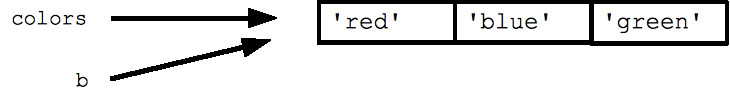
\includegraphics[width=4.16in,height=1.5in]{./uploads_new/SENDING_EMAIL.docx_DIR/media/image2.gif}
\end{center}
\end{figure}


 %%%%%%%%%%%%  Figure/Image No:2 Ends Here %%%%%%%%%%%%%%


\end{center}\vspace{12pt}
\noindent 
\begin{center}Gambar proses cara kerja mail server 1\end{center} \par
\vspace{12pt}
\noindent 
\begin{center}

 %%%%%%%%%%%%  Figure/Image No:3 here %%%%%%%%%%%%%%


\begin{figure}[H]
\begin{center}
\includegraphics[width=3.97in,height=3.26in]{./uploads_new/SENDING_EMAIL.docx_DIR/media/image3.jpg}
\end{center}
\end{figure}


 %%%%%%%%%%%%  Figure/Image No:3 Ends Here %%%%%%%%%%%%%%


\end{center}\vspace{12pt}
\noindent 
\begin{center}Gambar proses cara kerja mail server 2\end{center} \par
\vspace{12pt}
\vspace{12pt}
\noindent 
\textbf{Gambar proses cara kerja mail server 1} \par
\noindent 
\textbf{Cara Kerja Mail Server  $  \#  $Versi 2} \par
Cara kerja ini saya ambil dari Xmodulo, sebelum memahami proses cara kerja mail server sebaiknya anda mengenal terlebih dahulu singkatan - singkatan dari MUA, MTA, MDA dll. Berikut penjelasannya : \par
\vspace{12pt}
\noindent 
\begin{myEnumerate}
\item Mail User Agent (MUA) : MUA adalah komponen yang berinteraksi dengan pengguna akhir secara langsung. Contoh dari MUA yaitu Thunderbird, MS Outlook, Zimbra Desktop. Interface webmail seperti Gmail dan Yahoo juga MUA. \par
\noindent 
\item Mail Transfer Agent (MTA) : MTA bertanggung jawab untuk mentransfer email dari mail server mengirimkan sampai ke server penerima email. Contoh MTA yaitu sendmail dan postfix. \par
\noindent 
\item Mail Delivery Agent (MDA) : Dalam surat server tujuan, MTA lokal menerima email masuk dari MTA terpencil. Email tersebut kemudian dikirimkan ke kotak surat pengguna dengan MDA. \par
\noindent 
\item POP / IMAP : POP dan IMAP adalah protokol yang digunakan untuk mengambil email dari kotak surat penerima server untuk penerima MUA. \par
\noindent 
\item Mail Exchanger Record (MX) : Record MX adalah entri DNS untuk mail server. Catatan ini menunjuk ke alamat IP ke arah mana email harus ditembak. MX record terendah selalu menang, yaitu, mendapat prioritas tertinggi. Sebagai contoh, MX 10 adalah lebih baik daripada MX 20. Alamat IP dari MX record dapat bervariasi berdasarkan desain dan konfigurasi persyaratan, seperti yang akan dibahas nanti dalam artikel.\end{myEnumerate}
 \par
\vspace{12pt}
\noindent 
\begin{center}

 %%%%%%%%%%%%  Figure/Image No:4 here %%%%%%%%%%%%%%


\begin{figure}[H]
\begin{center}
\includegraphics[width=6.27in,height=2.16in]{./uploads_new/SENDING_EMAIL.docx_DIR/media/image4.jpg}
\end{center}
\end{figure}


 %%%%%%%%%%%%  Figure/Image No:4 Ends Here %%%%%%%%%%%%%%


\end{center}\vspace{12pt}
Ketika pengirim mengklik tombol kirim, SMTP (MTA) memastikan ujung ke ujung pengiriman email dari pengirim-sisi server ke server tujuan. Setelah mencapai server tujuan, MTA lokal ke server tujuan menerima email, dan di pindahkan ke MDA setempat. MDA kemudian menulis email ke kotak pesan penerima. Ketika penerima memeriksa email, mereka diambil oleh MUA dengan menggunakan protokol seperti POP atau IMAP. \par
\vspace{12pt}
\vspace{12pt}
\end{document}
